% !TeX root = ../thuthesis-example.tex

\chapter{故障场景高可用容错方案描述}\label{chap-failure-scenarios}

本章针对系统常见的故障场景,如磁盘写满、系统宕机、网络分区、集群变更等,分析了本文中提出的高可用和容错方案的支持。对于每一种故障场景,本章节都给出了错误的检测方法和容错恢复的方法。


\section{单节点磁盘写满}

\subsection{检测方法}

目前IoTDB集群中有两种单节点磁盘写满的故障检测方式。

第一种是定期预防式的诊断,通过管理节点和数据节点的心跳完成。管理节点和数据节点交换的心跳包中会带有该数据节点节点的磁盘最大容量和目前的使用情况。如果目前的使用率已经超过了预先设置的阈值,那么管理节点就会将该节点标志为只读的状态,标志着管理节点检测到了单节点磁盘写满的故障。

第二种是发生时的临诊,通过数据节点在写入过程中的自我检测来完成。在数据节点服务某一个写入请求,在文件系统上真正写入数据之前,会进行可写入性的检查。如果发现此时磁盘空间不足,那么本次写入请求就不会执行,并且返回给客户端本次节点只读的状态。

\subsection{高可用容错方案}

\begin{figure}
    \centering
    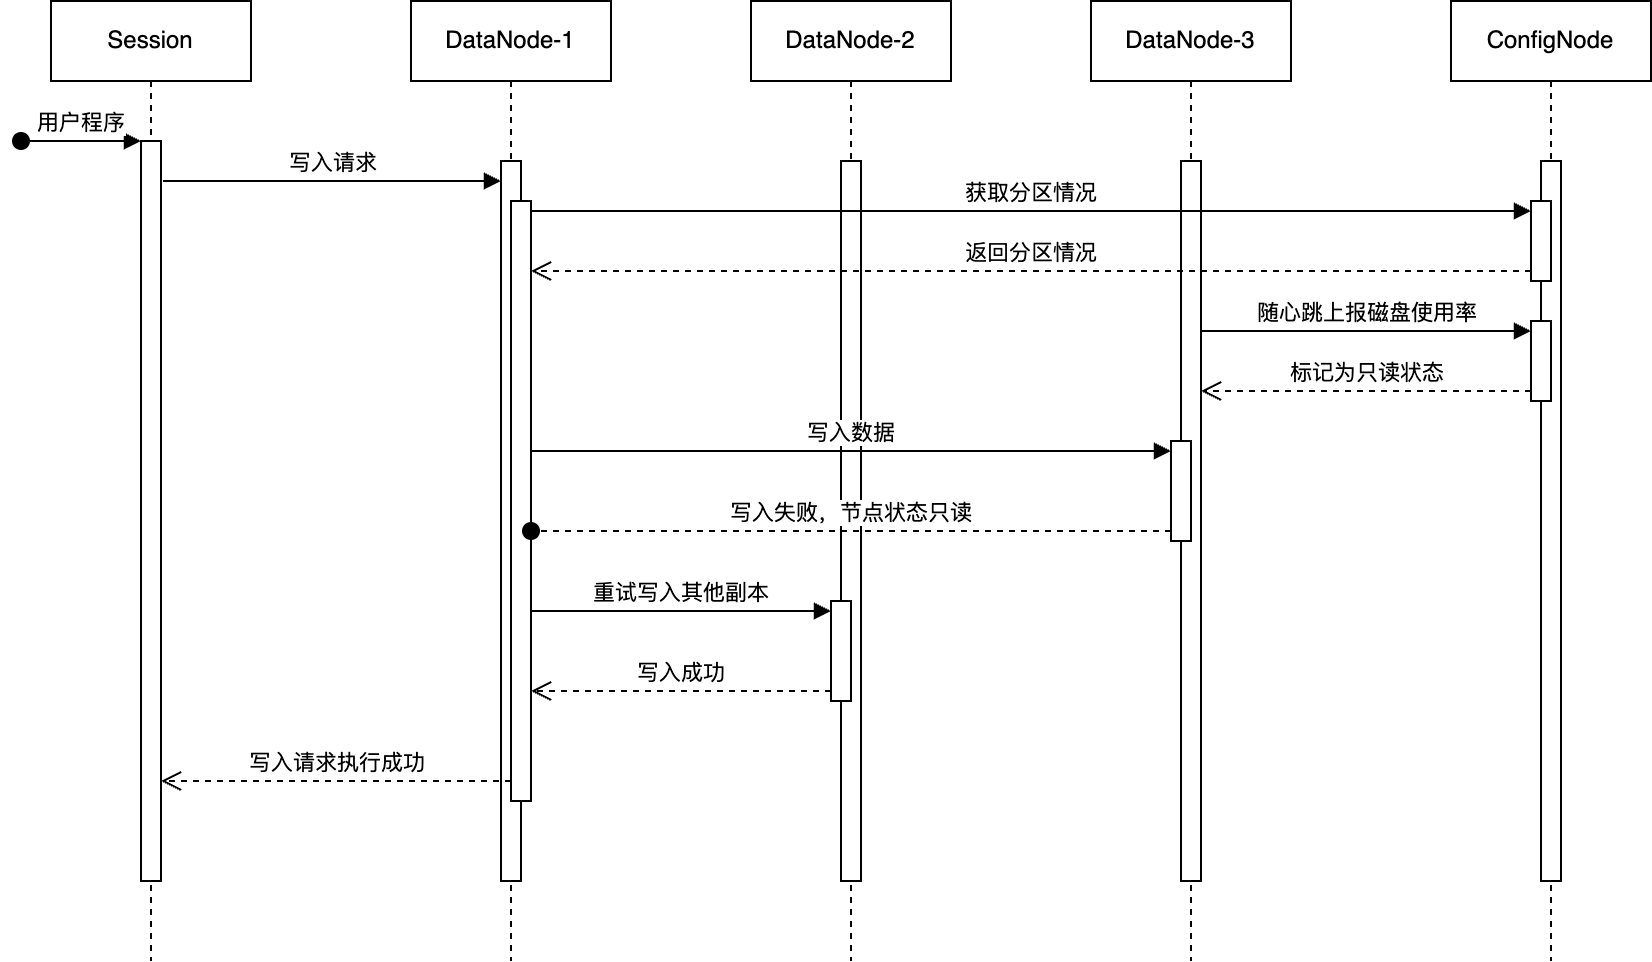
\includegraphics[width=0.99\linewidth]{c05-diskfull.png}
    \caption{单节点磁盘写满的高可用容错时序图}
    \label{fig:c05-diskfull}
  \end{figure}

图\ref{fig:c05-diskfull}给出了单节点磁盘写满的完整容错时序图。

可以看到,在某一个时刻,数据节点3的磁盘使用情况超过了阈值,并且在下一次和管理节点上报心跳的时候将这一情况上报给了管理节点。管理节点会将该节点标记为只读,这个信息会被同步到所有节点的协调者模块。

对于读请求来说,无论是故障发生时的在途请求,还是故障发生之后的新请求,都能够正常执行,不受任何影响。对于写请求来说,则通过前一章节描述的故障错误转移的方式来实现容错。

对于磁盘写满故障发生之后的写入请求,由协调者阶段在规划阶段进行容错处理。
在写入的规划阶段,规划器能够从管理节点获取最新的分区情况,明确了解该节点只读的状态,并会将本次的请求给路由到其他可以写入的副本上,从而完成写入请求的正常执行。

对于磁盘写满故障发生时就在执行的在途写入请求,通过协调者的调度阶段重试来实现容错。以图中的写入请求来说,请求在第一次规划时,数据节点3并未出现磁盘写满的故障,因此规划的结果是向这个数据节点3节点写入数据。
然而,在数据实际写入之前,数据节点3的状态变更为只读,无法服务这次的写入请求,因此本次的写入操作会返回异常。
数据节点1的协调者节点会捕捉到这次失败的调度,开启重试恢复。重试时,协调者会选择其他的可用副本所在节点(在本次请求中为数据节点2)尝试写入。由于数据节点2的状态健康,因此本次数据会写入正常运行的数据节点2中,最后实现数据的成功写入。


\section{进程宕机}

\subsection{检测方法}

IoTDB通过捕捉管理节点和数据节点之间维持的心跳信道断开这一事件,判断数据节点的进程宕机这一故障。

如章节\ref{thrift-detection}所述,管理节点领导者和数据节点之间的心跳通道是基于Thrift构建的,底层传输方式为Thrift的TSocket,这是一种基于TCP连接的传输。
当进程终止时,操作系统会立即关闭该进程打开的所有TCP连接。

管理节点领导者和数据节点之间建立的Thrift通道会因为进程宕机而断开,这一事件会被报告给管理节点领导者,从而使管理节点感知到节点宕机的故障。即使TCP连接没有立即断开,如果对端进程已经停止响应,任何尝试通过该连接进行读写操作都会导致I/O异常。Thrift框架也能够捕获这些I/O异常,例如连接超时、连接拒绝等,从而判断对端进程已失效。


\subsection{高可用容错方案}

在进程宕机的故障情况下,客户端会通过自动服务发现和转移的方式将客户端的请求流量引导到新的节点上,而协调者节点会通过调度时期的容错机制将内部的\fragmentinstance 引导到其他存活节点上的副本。

\begin{figure}
    \centering
    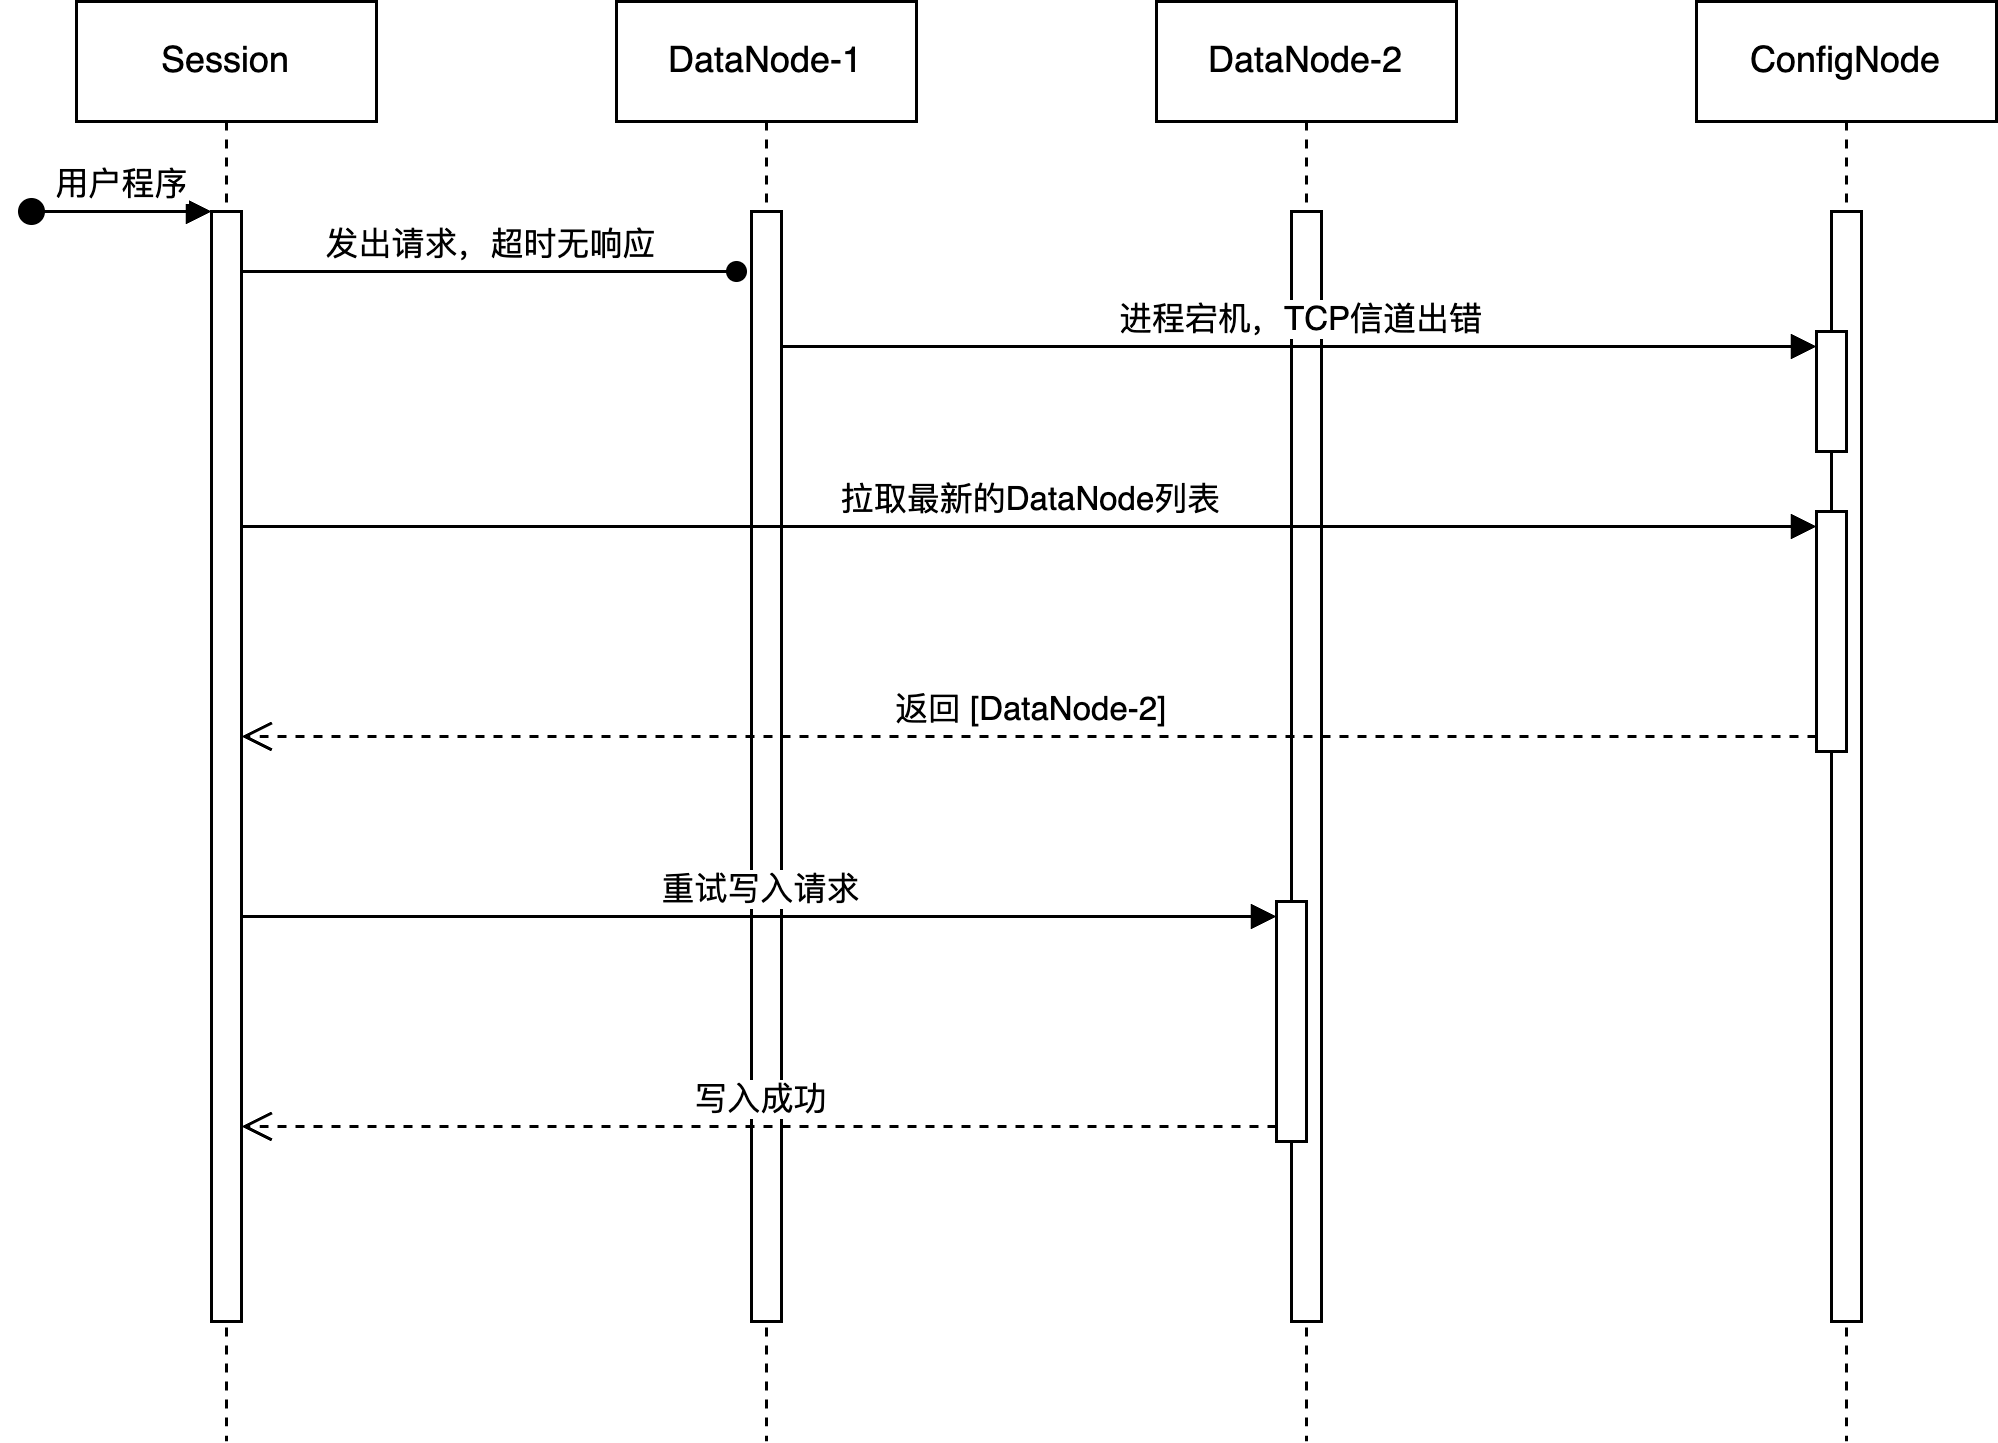
\includegraphics[width=0.99\linewidth]{c05-process-down-1.png}
    \caption{单节点进程宕机的高可用容错时序图}
    \label{fig:c05-process-down-1}
\end{figure}

图\ref{fig:c05-process-down-1}展示了客户端自动服务发现和转移的容错方案。图中数据节点1在处理客户端的请求的时候出现了宕机,会导致客户端的该请求超时无响应。

一方面,管理节点通过Thrift信道的连接断开事件检测到数据节点1节点的进程异常,并会更新这个节点的状态。由于客户端的后台进程会持续地从管理节点拉取最新的数据节点列表,因此在下一次拉取的时候,客户端就能够发现数据节点1失效的问题。

另一方面,客户端会尝试向其他的数据节点进行请求重试,在本例中会将请求数据引导到数据节点2上。由于此时数据节点2正常工作,因此本次请求能够被正常处理,从而使用户的请求最终能够正常写入。


对于集群内部的请求流量,例如其他节点的协调者模块发送到本数据节点1上的\fragmentinstance ,会由其他节点的协调者重试其他的数据副本,重试的算法和前一章节磁盘写满的流程图\ref{fig:c05-diskfull}相似。

\section{对称网络分区}

\subsection{检测方法}

IoTDB通过依赖管理节点和数据节点之间交换心跳包,根据心跳历史和Phi Accrual研判算法来检测对称网络分区。

当节点发生对称网络分区的时候,由于节点依旧存活,操作系统不会关闭TCP信道,因此我们需要依赖心跳历史的采样进行研判。由于管理节点之间会持续交换心跳,在超过一定的时间之后,Phi Accrual算法就会研判该数据节点不可达,管理节点领导者将会将该节点的状态设置成不可知。


\subsection{高可用容错方案}

对于发生非对称网络分区的数据节点,在事实意义上可以认为这个节点完全不可用。因此,在容错方案上,可以借鉴上一小节进程宕机的处理方法。

对于连接在该节点上的客户端,可以通过\ref{fig:c05-process-down-1}所示的流程将请求流量引导到其他不分区的数据节点上。

对于协调者内部的\fragmentinstance ,可以通过\ref{fig:c05-diskfull}所示的流程将请求流量引导到其他非分区存活副本所在的数据节点上。


\section{非对称网络分区}


\subsection{检测方法}

IoTDB通过数据节点之间的对等心跳来检测非对称网络分区的故障。在非对称网络分区的情况下,由于所有的数据节点依然能够和管理节点之间正常交换心跳包,因此无论是通过Thrift心跳通道,还是通过管理节点的心跳和研判算法都无法检测出非对称网络分区的故障。

此时,需要通过章节\ref{sec:数据节点-intra-heartbeat}所述的数据节点之间的对等心跳来检测。
数据节点之间会定期和所有的其他数据节点之间交换心跳,验证连通性。如果数据节点1和数据节点2发生了非对称网络分区,那么数据节点1和数据节点2之间无法进行心跳交换。数据节点1和数据节点2分别会将这个情况上报给管理节点领导者。管理节点领导者会通过Phi Accrual算法分析对等心跳,并且研判出数据节点1和数据节点2之间出现了非对称网络分区的问题,实现故障的检测。


\subsection{高可用容错方案}

IoTDB通过协调者在规划阶段的容错和客户端侧的协同来共同解决非对称网络分区的问题。

\begin{figure}
    \centering
    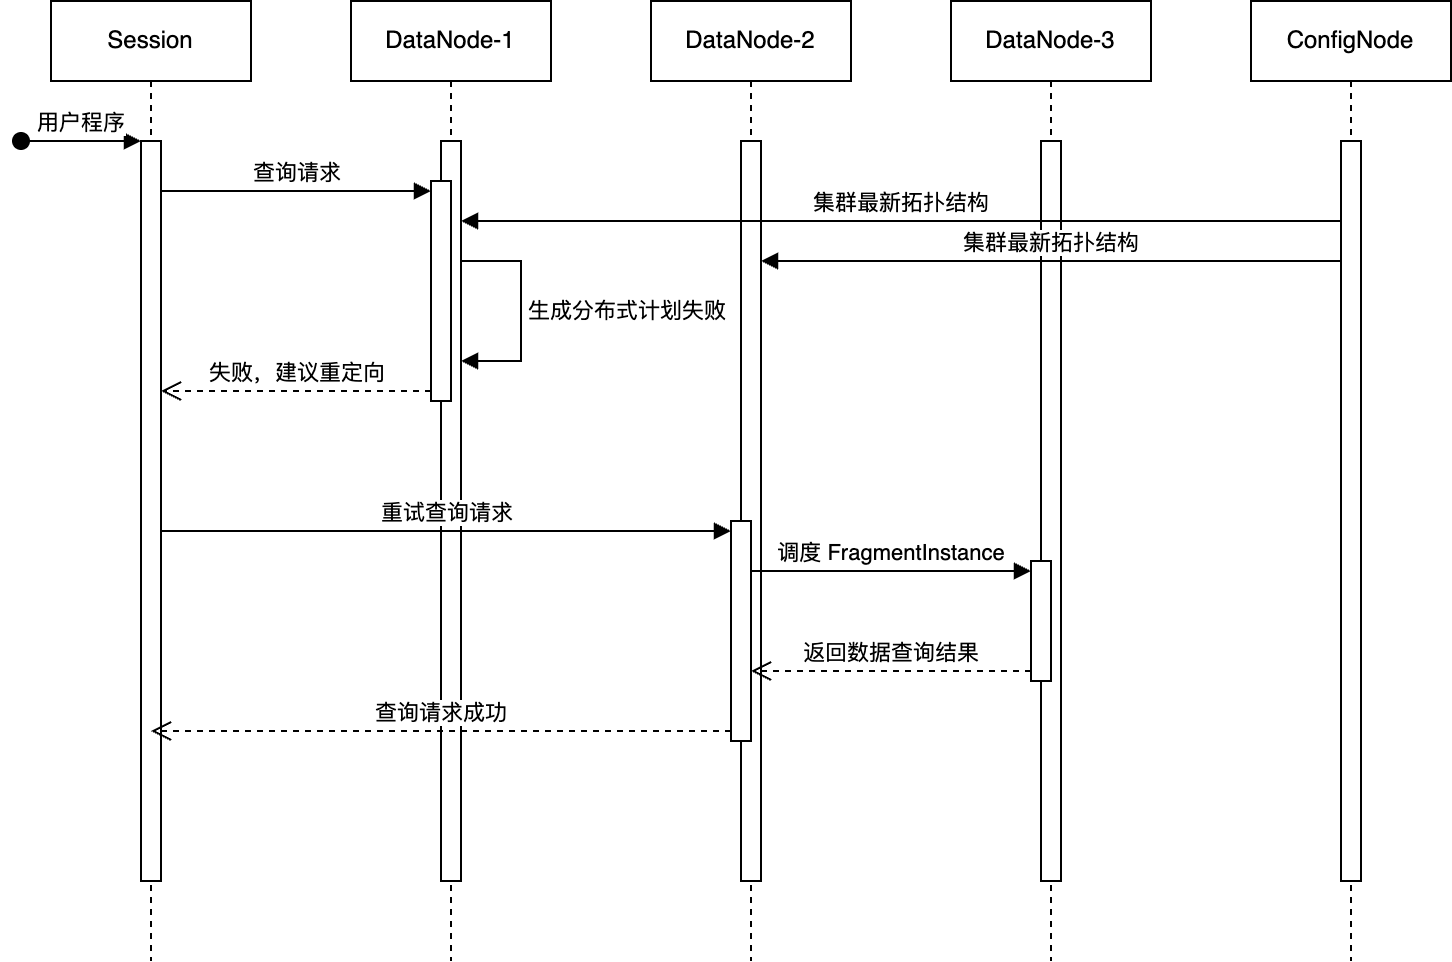
\includegraphics[width=0.99\linewidth]{c05-partition-asym.png}
    \caption{非对称网络分区的高可用容错时序图}
    \label{fig:c05-partition-asym}
\end{figure}

图\ref{fig:c05-partition-asym}给出了非对称网络分区的高可用容错时序图。假设集群数据节点1和数据节点3之间出现了非对称网络分区。当客户端连接到数据节点1上并发送了查询请求,在数据节点1上的协调者会解析规划这个查询请求。假设这次查询请求的\fragmentinstance 将会被调度到所有的数据节点1、数据节点2、数据节点3上,此时根节点的\fragmentinstance 必须被调度到能同时和三个节点的联通的数据节点,即数据节点2上。因此,本次规划会立即失败,向客户端返回失败的状态码,并建议客户端将请求重定向到数据节点上执行。

客户端在遇到失败的状态码的时候,会重新将请求定向到数据节点2上执行。由于数据节点2并不存在网络分区的问题,能够与集群内的所有节点正常连接,因此查询规划能够顺利生成和调度,在三个数据节点之间进行数据的实际查询和数据聚合,完成本次的查询请求,将结果返回给客户端的客户端。

\section{管理节点节点脑裂}

管理节点是集群的大脑,负责管理集群的节点基础信息、当前状态、集群的拓扑网络结构、集群的分区信息等,并且管理节点上运行着诸多后台的服务,包括负载均衡、分区迁移等服务。
为了保证
管理节点服务的高可用,我们会同时运行多个管理节点的副本,每一个副本都保持了相同的数据,但是同一时刻只能有一个主副本发号施令,决定服务的实际状态。当主副本所在的管理节点节点出现宕机的时候,其他的副本则会通过选举流程产生一个新的主副本,接替相关的任务。

如果主副本短暂地发生了网络分区的情况,其他副本如果此时发起选举并且被正式选举为主副本,此时旧的主副本的网络分区恢复,且旧的主副本还没有意识到自己已经不再是领导者的情况下,就会导致集群中有两个主副本同时发号施令,从而出现所谓的脑裂情况。

\subsection{检测和容错方案}

我们通过设置主副本的租约和从副本的最小选举超时时间来避免出现脑裂。


管理节点的领导者副本需要持有租约才能提供服务。
租约可以认为是一个带时效的排他锁,表示在一个时间内只有一个特定的节点能够成为领导者,提供领导者的服务。
在IoTDB集群中,租约的持续时间为80\%的最小心跳超时。
假设心跳最小超时为5s,最大超时为10s,
那么租约的持续时间为4s。这意味着。当一个节点当选为管理节点领导者之后,自动拥有了4s的领导者租约,表明在接下来的4s内能够安全行使领导者的权力。每当管理节点领导者通过心跳获得了大多数的拥戴之后,租约的时间就会向后延期4s。
如果管理节点领导者在4s内都没有获得大多数节点的心跳回复,那么本次的租约失效,领导者将失去身份,不得开展相关的活动。

这样的机制保证了不会有两个领导者同时开展活动。在网络分区的情况下,被分区的领导者在4s之后就会自动失去领导者身份,而下一任的领导者至少需要5s才能被选举出来,中间的时间差有效避免了脑裂问题的发生。

这种机制虽然安全地防范了脑裂问题的产生,但会导致管理节点领导者服务会有1s时间的短暂不可用。因此,客户端和协调者节点在请求
管理节点节点的服务时,也需要具备一定的重试和容错的方案。

\begin{figure}
    \centering
    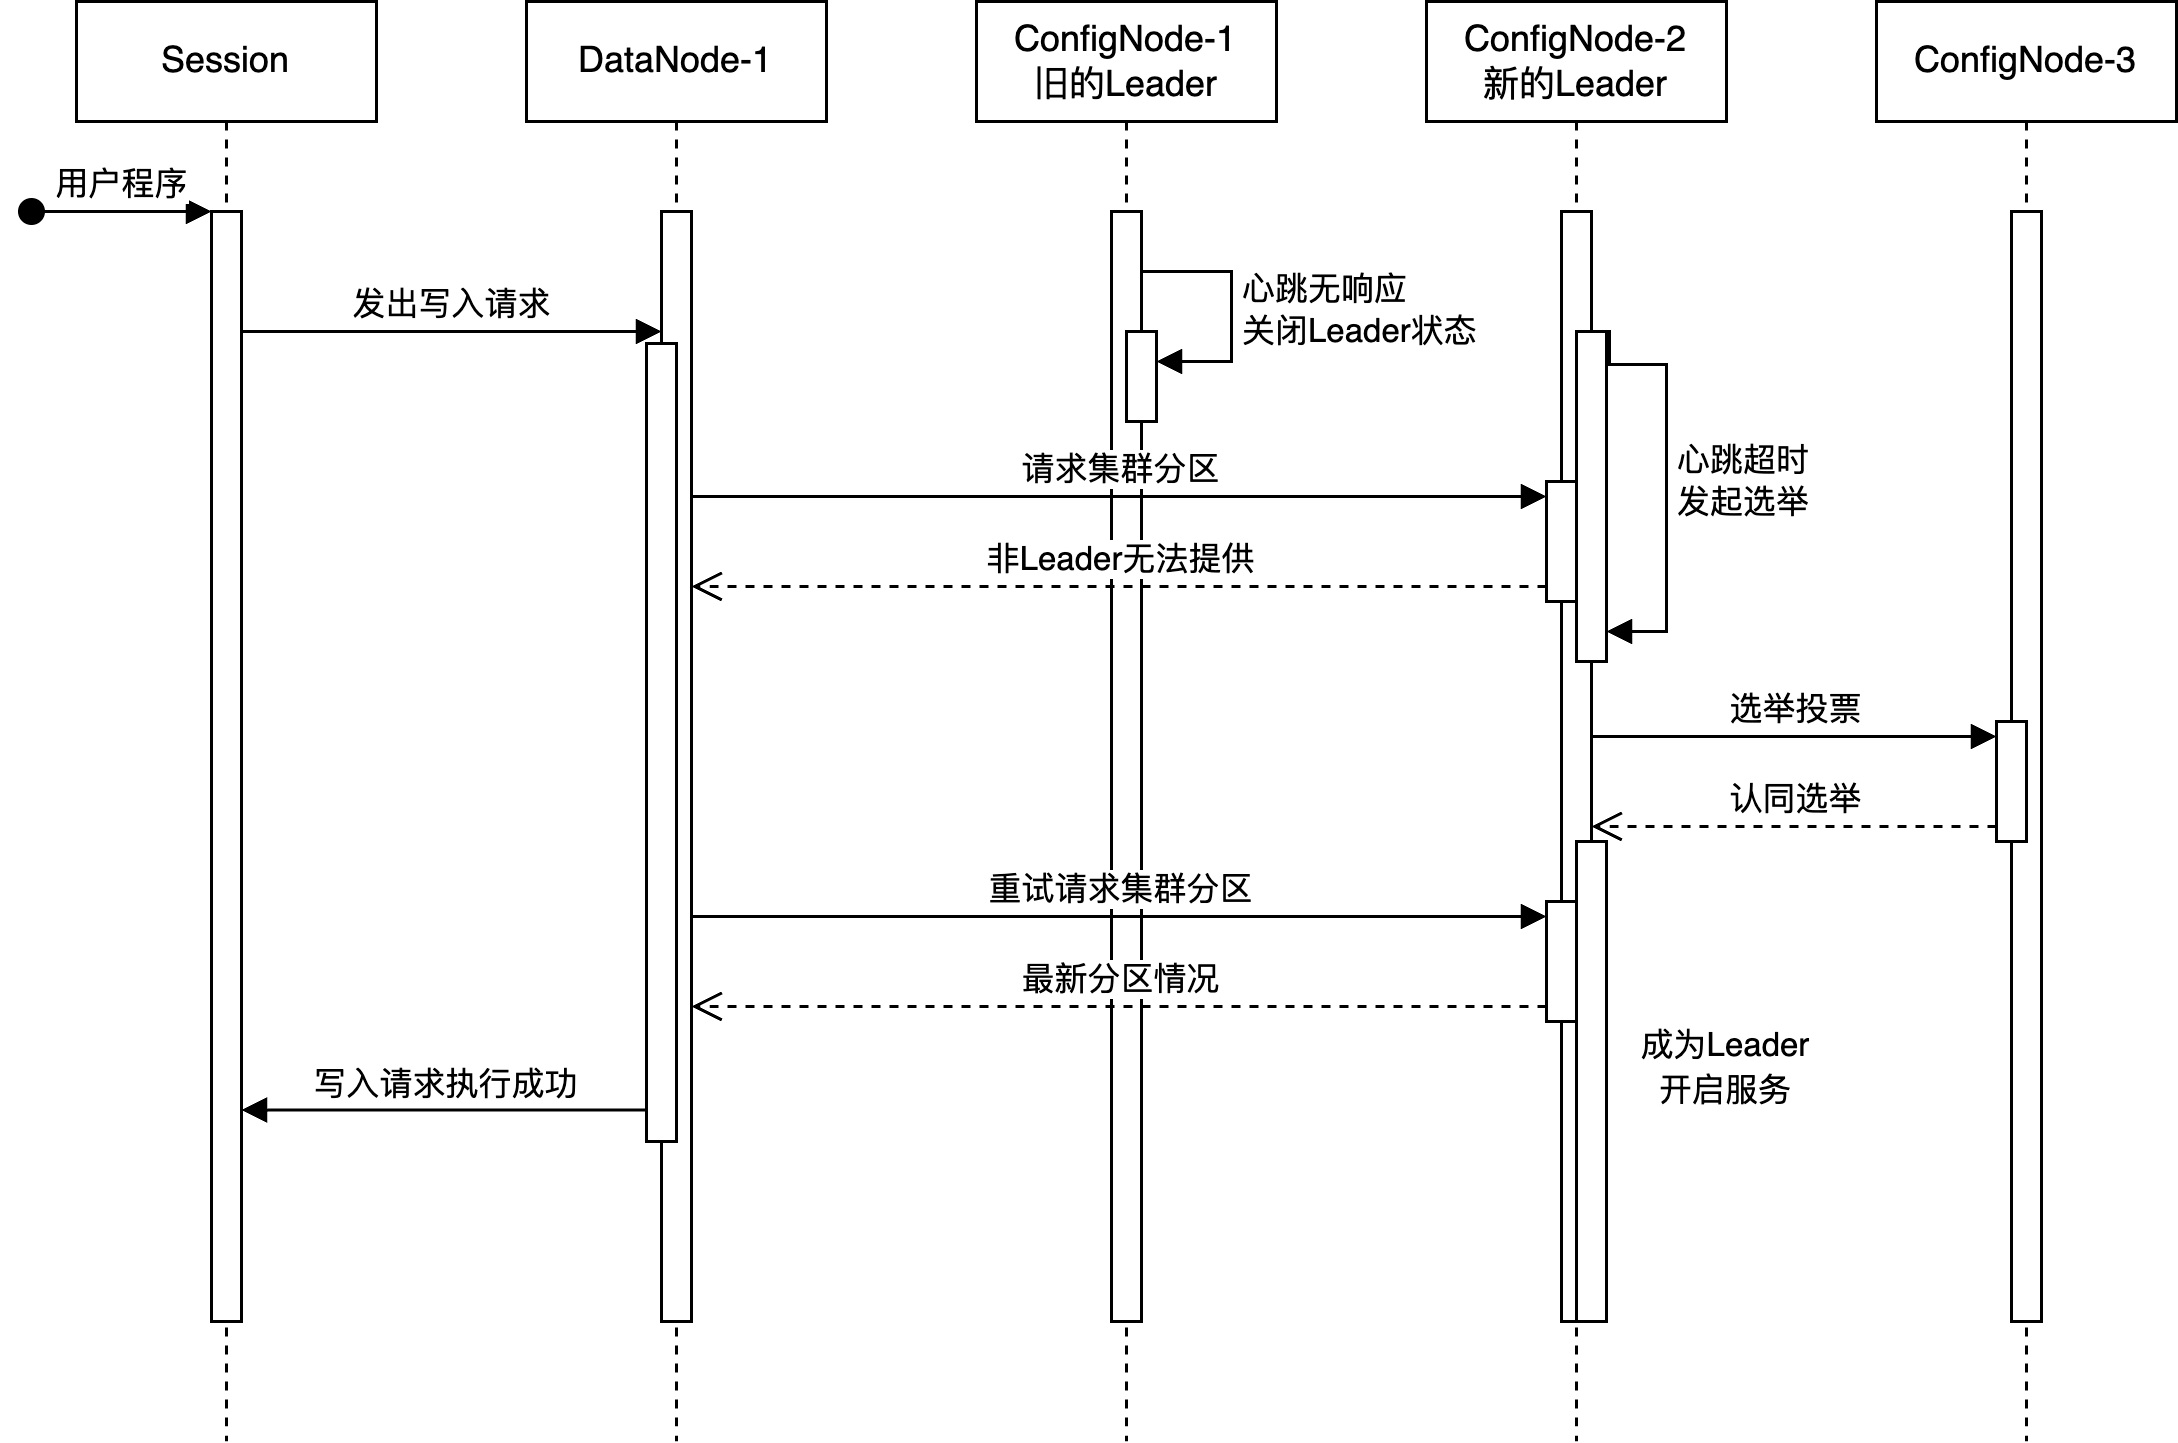
\includegraphics[width=0.99\linewidth]{c05-brain-split.png}
    \caption{管理节点服务的高可用容错时序图}
    \label{fig:c05-brain-split}
\end{figure}

图\ref{fig:c05-brain-split}展现了管理节点因为短暂的网络分区而导致服务不可用的情况下的高可用时序图。其中,管理节点1是旧的领导者,由于和剩下的两个副本管理节点2/管理节点3之间出现了网络分区,导致在一段时间心跳无响应的状态下失去了租约,主动结束了领导者的服务。此时集群中没有管理节点节点能够提供服务。

此时,如果用户的写入和查询请求需要向管理节点获取分区等服务,那么这些请求就无法得到响应。比如,数据节点2需要等待一段时间,再进行重试。

在等待的这段时间里,管理节点2率先出现选举超时,开始新一轮的选举,并在管理节点3的支持下成功当选最新一期的领导者,并正常开启了管理节点 的服务。此时,数据节点2再重试请求分区,管理节点2能够正常对其提供服务,数据节点也能够顺利完成请求的执行。


\section{集群变更状态下的一致性}

\subsection{错误检测}


IoTDB在不对集群变更进行错误检测,系统通过客户端侧的重试和协调者侧的重试来对数据不一致的问题进行容错。


\subsection{高可用容错方案}

\begin{figure}
    \centering
    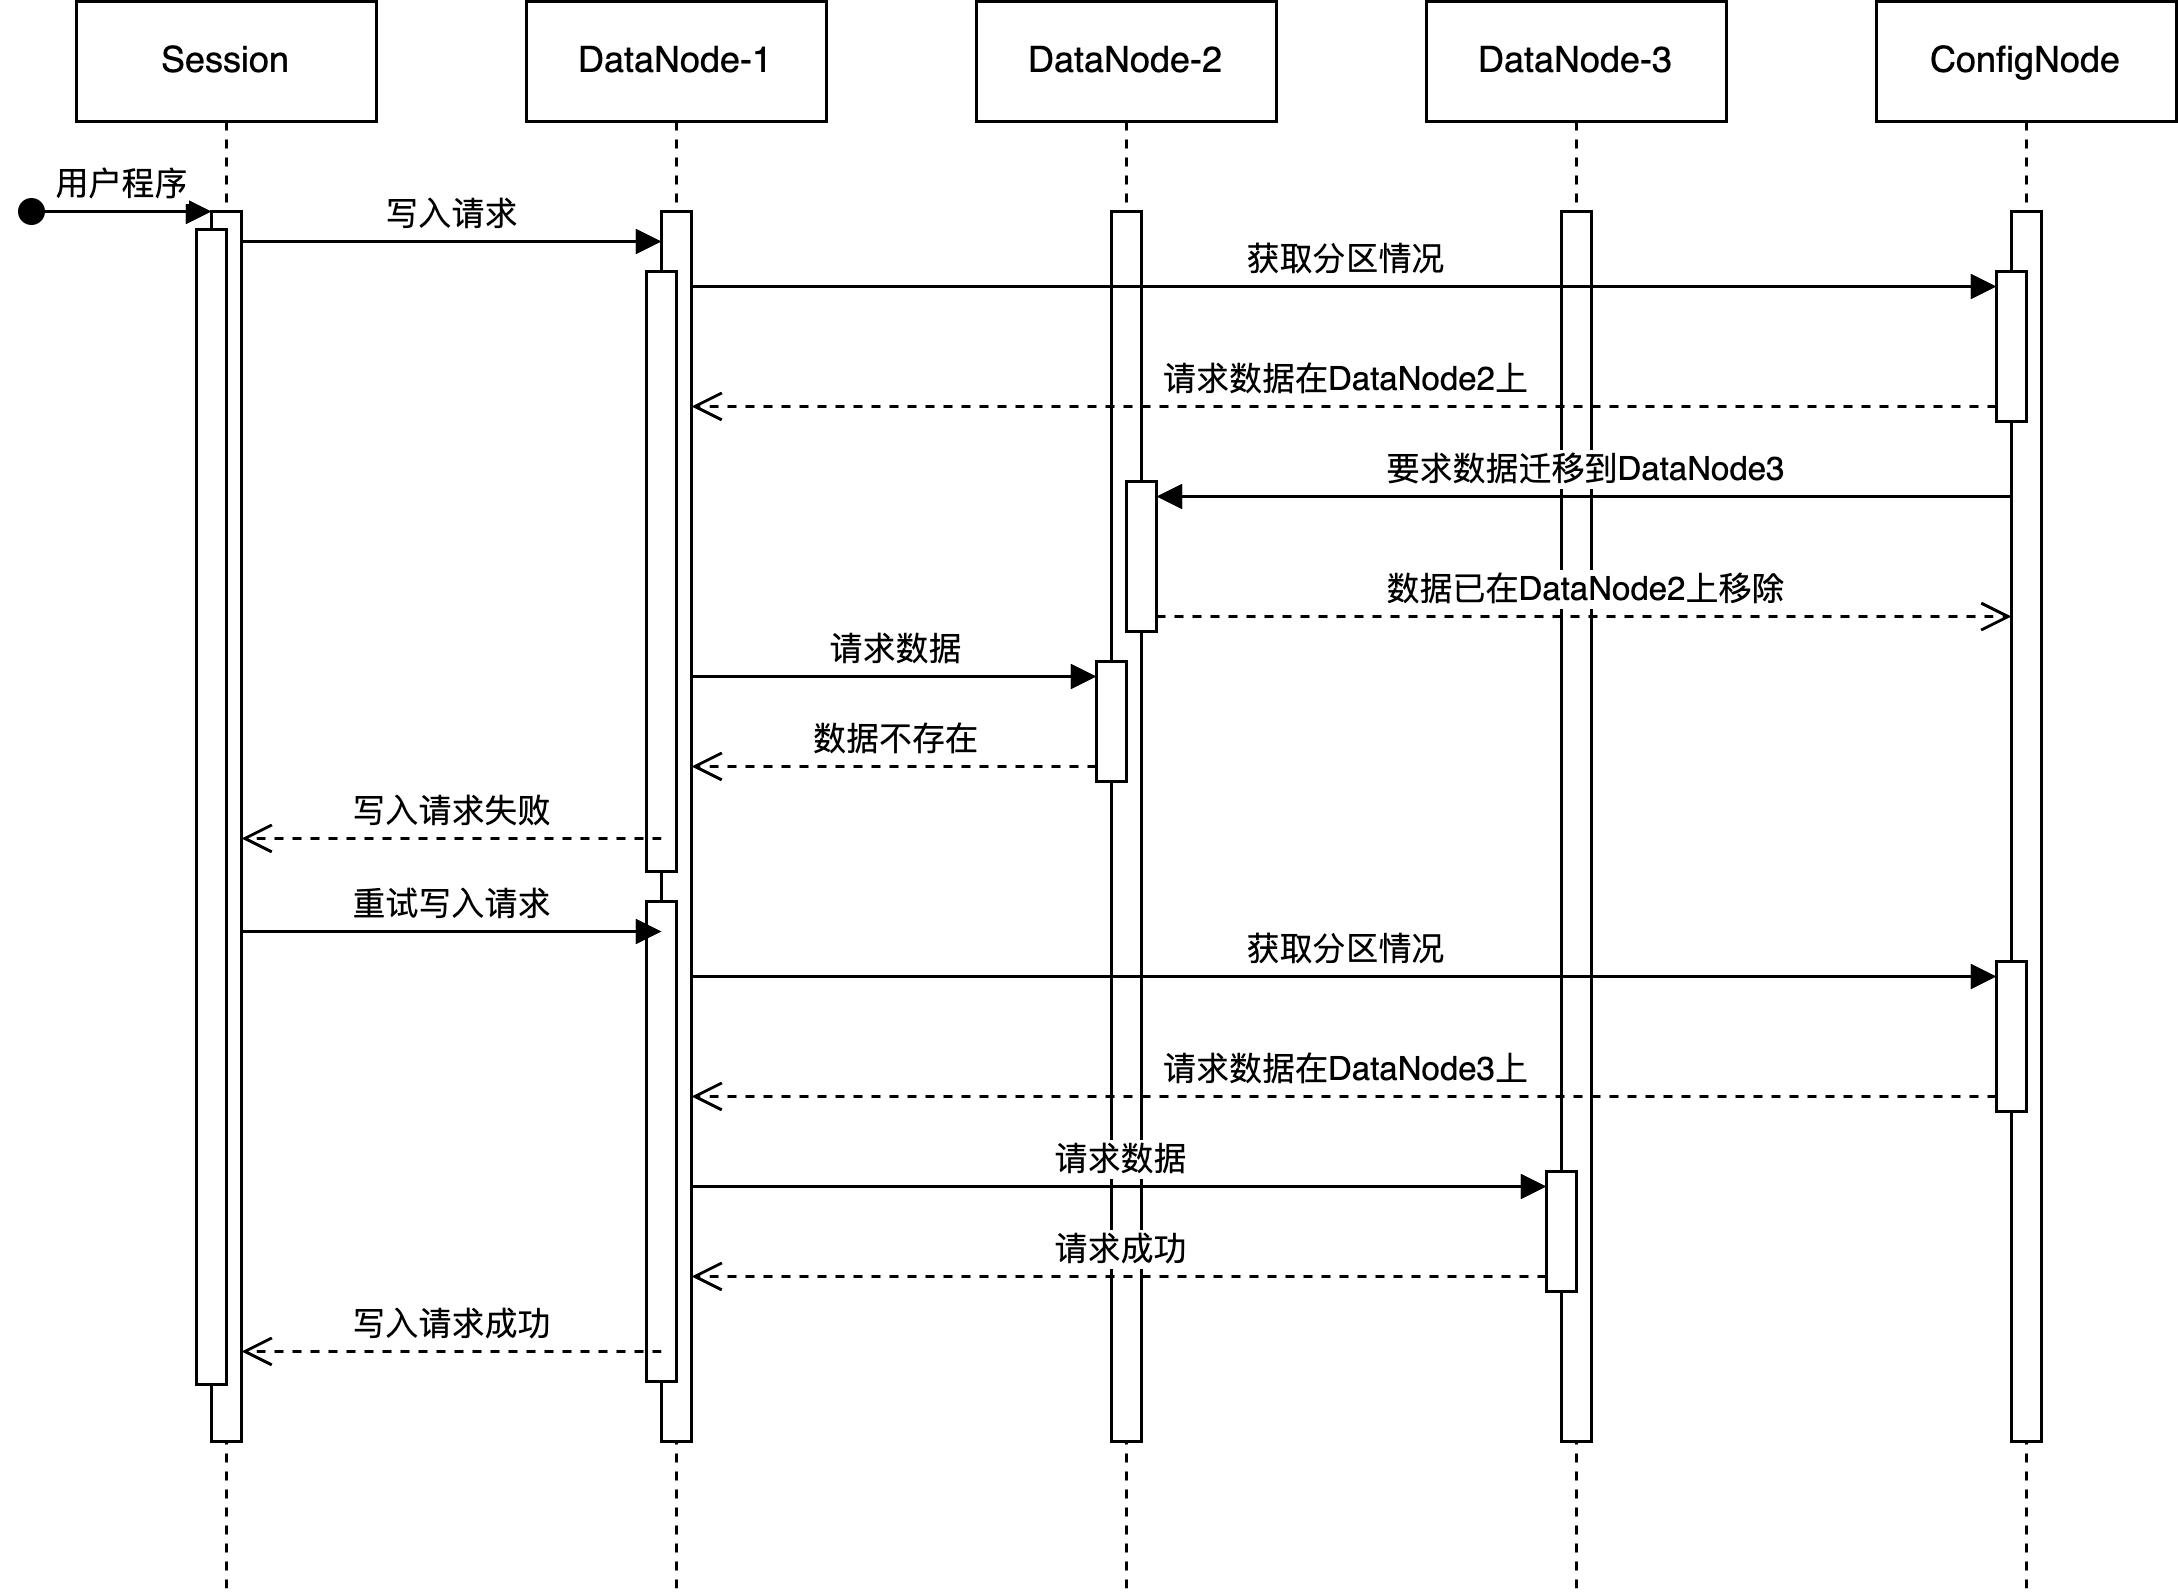
\includegraphics[width=0.99\linewidth]{c05-cluster-change.png}
    \caption{集群变更状态下高可用容错时序图}
    \label{fig:c05-cluster-change}
\end{figure}

图\ref{fig:c05-cluster-change}展示了在集群变更状态下系统的高可用容错时序图。用户在通过客户端进行写入请求的时候,数据节点1先从管理节点领导者这里获取了分区情况,发现所请求的副本存活在数据节点2上,并根据这个分区情况进行写入规划。
然而在规划完成之后,调度执行之前,处于负载均衡或者扩缩容的考虑,管理节点领导者决定进行分区迁移,将原本在数据节点2上的数据副本迁移到数据节点3上。这导致在调度执行的时候,协调者节点依然会向数据节点2上已经不存在的“影子副本”发出请求。
此时,该请求会因为数据不存在而失败,数据节点2会拒绝本次请求,并且附上重试的建议。
如果本分区有多个数据副本,那么协调者节点会首先请求其他的数据副本。在本例中,该分区只有一个副本,因此数据节点1上的协调者节点只能将这次请求失败的信息返回给客户端,并且附上重试的建议。
客户端会在等待一段时间之后继续重试这个请求。这导致了请求会再次被发送到数据节点1上。此时,数据节点1会再次从管理节点这边获取最新的分区情况。此时最新的分区已经能够反映上次迁移的改变,因此数据节点1能够正确认识到数据此时存活在数据节点3上,从而向数据节点3发起请求,最终成功获取数据,本次写入也能顺利执行。

\section{本章小结}

本章深入分析了 Apache IoTDB 分布式系统中常见的多种经典故障场景,包括单节点磁盘写满、进程宕机、对称及非对称网络分区、管理节点 脑裂以及集群变更状态下可能引发的短暂不一致性问题。

针对每一种故障场景,本章详细阐述了高可用框架的故障检测能力如何对上述故障有效检测,包括基于心跳的阈值检查、进程连接状态监听、数据节点间的对等心跳以及管理节点的领导者租约机制等。

本章详细阐述了高可用框架在这些具体故障场景下的应用和应对策略。容错方案普遍依赖于管理节点对集群状态的准确感知和同步,客户端的自动服务发现和请求重试,以及数据节点内部协调者在规划和调度阶段的智能重试与副本选择。通过这些组件的协同工作,系统能够在面对上述复杂故障时,实现用户请求的自动路由、重试和恢复,从而保障分布式时序数据库的高可用性和数据一致性。本章的分析和时序图展示了这些容错机制在实际运行中的具体流程。